\documentclass{article}
\usepackage[utf8]{inputenc}
\usepackage{graphicx}
\usepackage{subfig}
\usepackage{float}
\usepackage{hyperref}

\title{Time Cube}
\author{Tomáš Havlík (havlito5@fel.cvut.cz)\\B4M39PTV}
\date{3.6.2018}

\begin{document}

\maketitle

\tableofcontents

\newpage

\section{Motivation}

One of the most prominent first-world issues of the 21st century is that of lack of focus and procrastination. One of the effective ways to fight this issue is to use a time tracker. Unfortunately, most time trackers are software-based and increasingly are accessed via a web browser, which often leads to the user straying from the task they are supposed to be doing. Would not it be great if we had a hardware device that allowed the user to stay focused on the task at hand?\\

Another great technique to increase focus that the author uses personally is called \textit{Pomodoro}, it involves setting a timer during which the user is supposed to be working on a task and forcing them to take a short break after the time runs out.\\

\section{Target demographic}

We believe that the product has a universal appeal and thus should be usable by as many people as possible. We would like to make it accessible to everyone with basic motor skills.

\section{Scenario}

In this chapter we will look at two fictional human beings that struggle with keeping focus.

\subsection{Alice}

Alice is currently studying for exams. Her schedule for next week includes three courses - cryptography, psychology and Japanese. She is desperate and struggles to maintain focus, instead jumping erratically between the slides for her three courses.

\subsection{Bob}

Bob is a self-employed full-stack software developer. He wants to find a solution that helps him manage his time better as he has a rather harmful tendency to play his favorite game for hours on end and binge-watch movies on Netflix, forgetting about his work in the process. Because he works from home, he needs to find a tool that helps him mentally separate time for work from off-time.

\newpage

\section{Requirements}

When coming up with the design we have set the following requirements for the product:

\begin{itemize}
\item Utilize a simple, intuitive interface.
\item Integrate Pomodoro functionality.
\item Allow for easy modification of activities.
\item Minimize cognitive load during use, allowing the user to focus on task at hand.
\item Allow the user to build the product using off-the-shelf parts and at a low cost.
\item House all necessary electronic devices.
\end{itemize}

\section{Design}

We have split this chapter into two subsections. The former talks about the physical model while the later goes through the design of the companion application.

\subsection{Hardware}

The cube's edges measure 4 centimeters in length. Dimensions of the cube were selected to fit all electrical components that are required for our cube to operate. These include the following:

\begin{itemize}
\item CR2032 battery cell (20 x 20 x 2 mm)
\item BLE Nano V2 system on a chip (18.5 x 21 x 4 mm)
\item ADX L355 accelerometer module (20 x 15.5 x 4 mm)
\item 3V vibration motor (10 x 10 x 3 mm)
\end{itemize}

In addition to the electronics, we also had to factor in the thickness of the walls as well as the margin of the battery compartment. Although the Bluetooth Low Energy standard should reduce the need to change batteries, we wanted to make the process as simple as possible. The circular cap that covers the battery compartment has an indent that fits the CR2032 battery to provide extra grip, which translates to better torque.

\newpage

\begin{figure}[H]
\centering
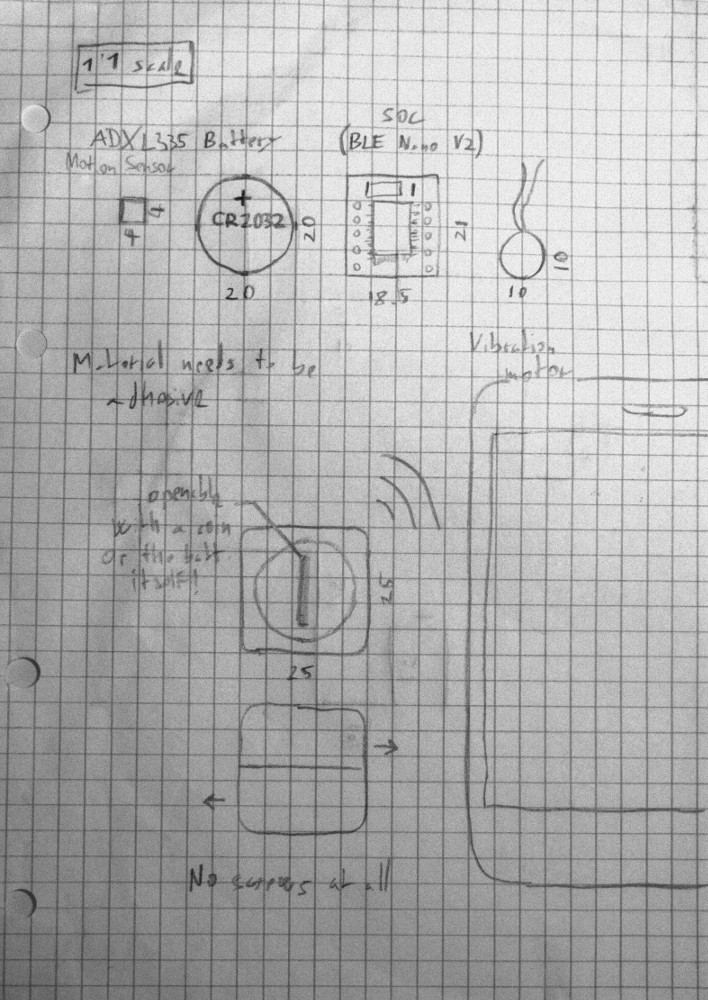
\includegraphics[scale=2.25]{draft.jpg}
\caption{Original draft. Note the smaller dimensions of the cube. Furthermore, ADX L355 dimensions are for the chip only.}
\label{fig:draft}
\end{figure}

\newpage

\begin{figure}[H]
\centering
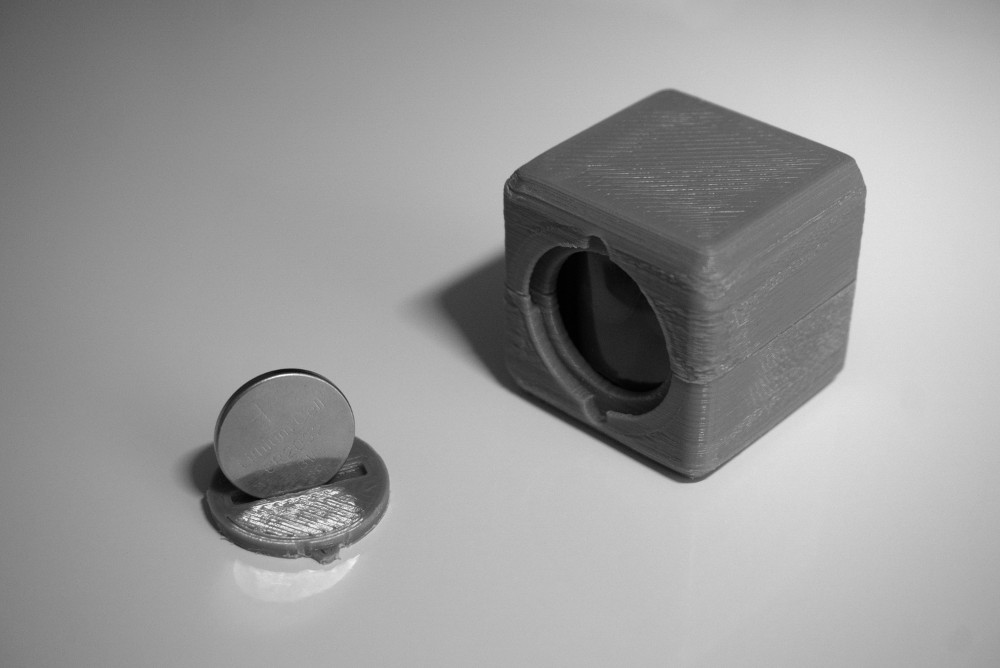
\includegraphics[scale=1.6]{cube_overview.jpg}
\caption{The cap can be opened using a CR2032 battery.}
\label{fig:cap}
\end{figure}

The indent also functions as a visual cue as the face which houses the battery compartment is used when the user wants to pause tracking and activate standby mode. Alternatively a cross-shaped visual cue could be used.\\

The five remaining faces contain no features whatsoever, allowing the user to attach stickers corresponding to activities detailed in the following section. The product can be further customized to enable use by those with poor or no vision via the utilization of special tactile stickers that contain bumps corresponding to braille characters or shapes.\\

Our design philosophy was to keep the amount of I/O on the cube itself to a minimum in order to allow the user to integrate it into their natural work flow and avoid distractions caused by flashing LEDs and like. The sole input method available to the user is rotation. Current activity is selected depending on the cube's orientation. The cube also includes a single output device - the vibration motor. Short pulses of vibration are triggered when the Pomodoro timer reaches a set amount of time.

\newpage

\begin{figure}[H]
\centering
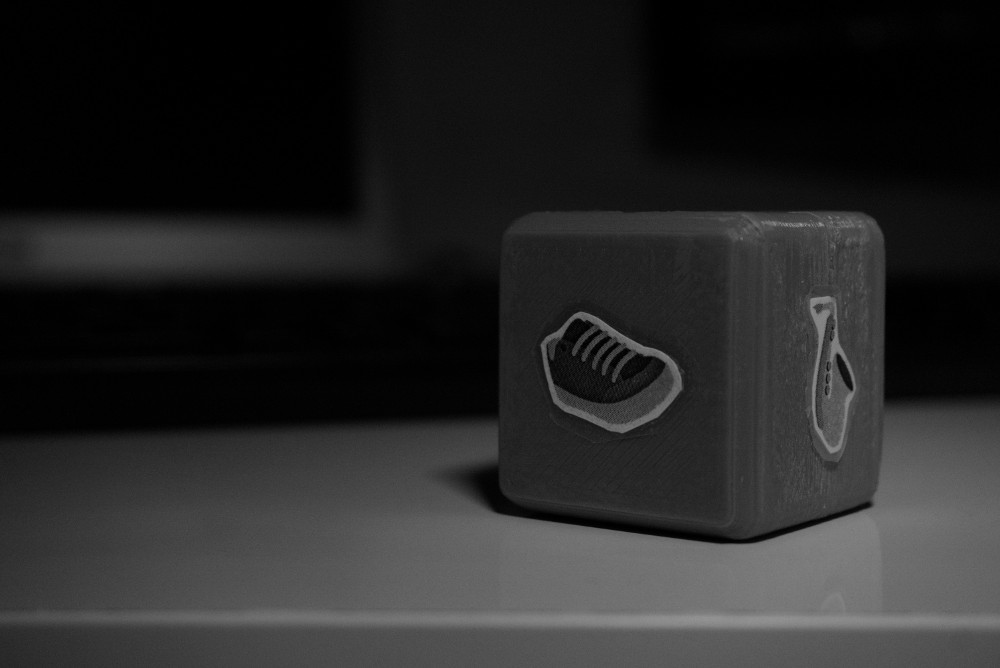
\includegraphics[scale=1.6]{cube_sides.jpg}
\caption{Stickers can be attached to any of the remaining five faces.}
\label{fig:stickers}
\end{figure}

\begin{figure}[H]
\centering
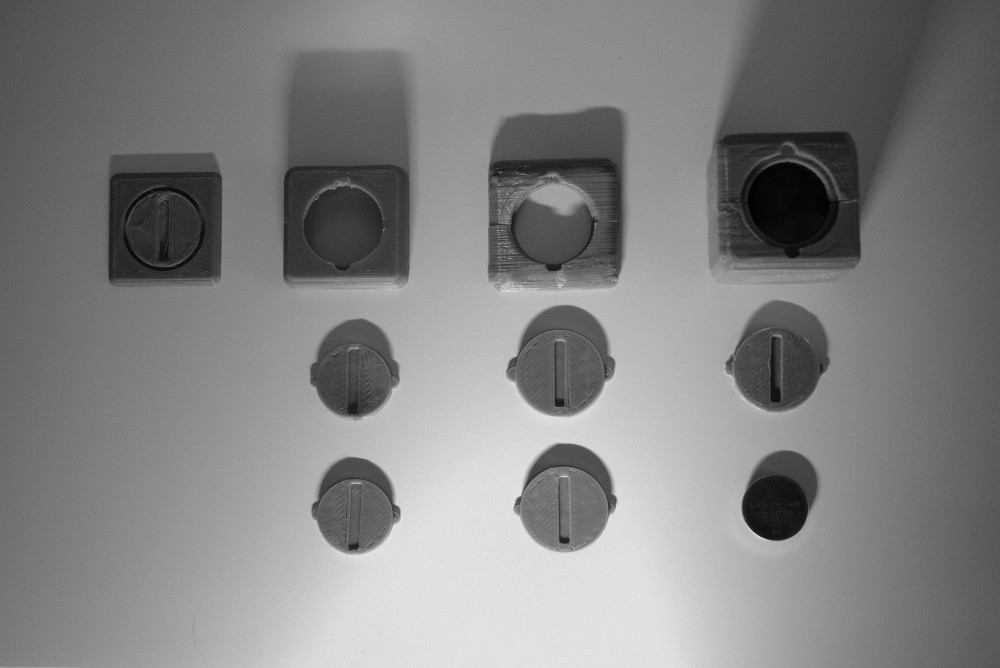
\includegraphics[scale=1.6]{cube_flow.jpg}
\caption{Iterations on the battery cap mechanism.}
\label{fig:history}
\end{figure}

\newpage

\subsection{Companion application}

As a part of the design process, we have designed an application that serves three functions. The first is to provide an overview of user's activity. The user can toggle between multiple graph views and time periods. We have tried different approaches to user interaction and decided to use a design that respects iOS guidelines in regards to page controls. Swiping horizontally switches the view and swiping vertically changes the position in time.\\

The second important function our application provides is the ability to modify activities. These activities are visually represented by icons. Color codes are assigned to activities depending on the prevalent color of selected icon and used in graphs, which maximizes clarity and allows us to achieve a minimalist, yet coherent interface. Icons in the application are physically represented with stickers that the user prints out and attaches to their cube. If the user is not satisfied with included stickers, they are able to take a photo of their own design.\\

The last function of our application is to allow the user to associate a Pomodoro timer with some of their activities. Tapping the activity icon activates or disables the timer and dragging the finger around a clock face changes the timer's duration.\\

To help the user get started, we have designed a new user experience, which goes through the process of installing a battery cell, wireless pairing and teaching the user that they can change the current activity by rotating the cube. Afterwards they are instructed to personalize their cube by selecting an activity.

\begin{figure}[H]
\centering
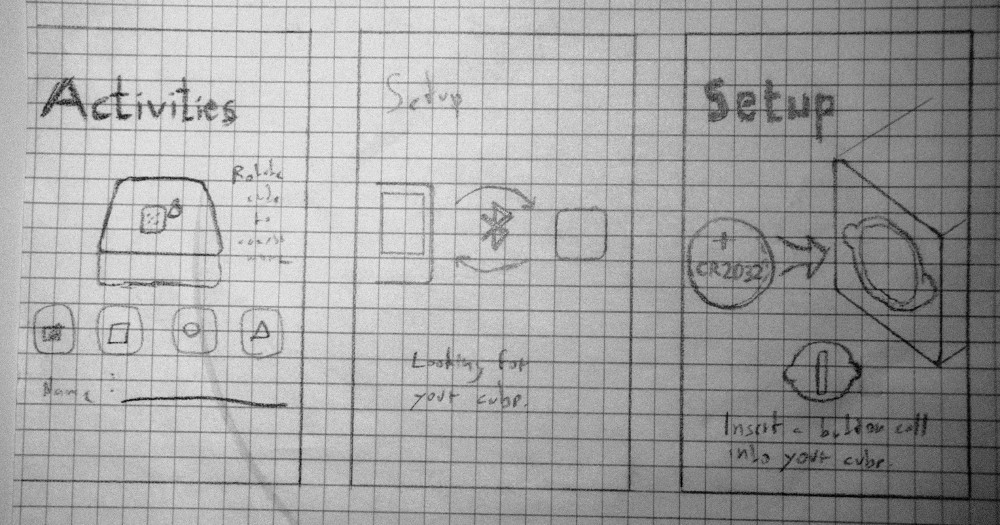
\includegraphics[scale=1.6]{draft_intro.jpg}
\caption{Rough draft of the setup procedure.}
\label{fig:draft2}
\end{figure}

\newpage

\begin{figure}[H]
\centering
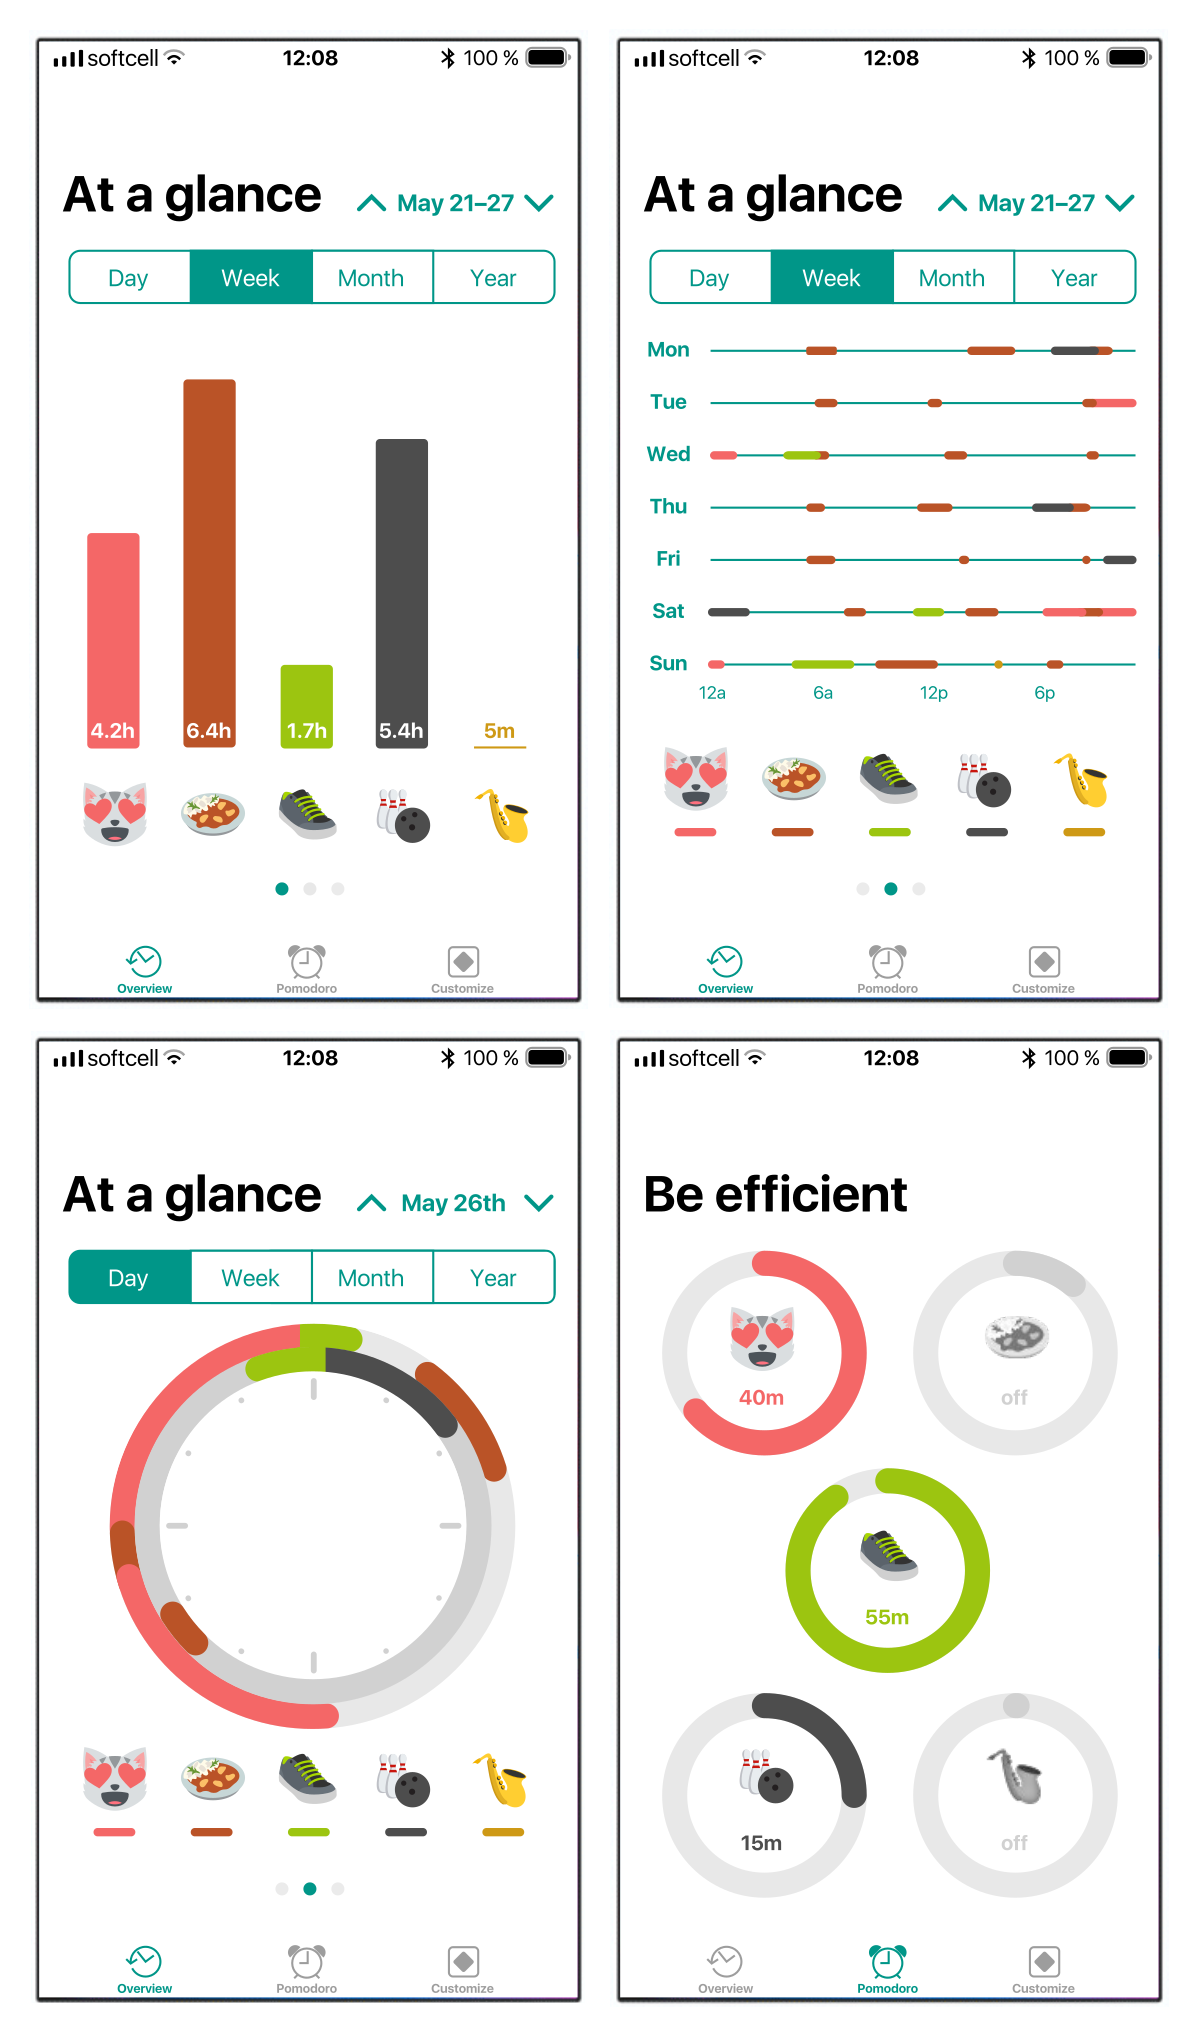
\includegraphics[scale=1]{app_screens.png}
\caption{Prototype of the application interface. Further depictions of the setup process and customization section are available in \textit{app\_prototype.pdf}, which should come bundled with this document. }
\label{fig:app}
\end{figure}

\newpage

\section{Technology}

In accordance with the open-source hardware philosophy, we want to give the end user the ability to construct their time cube from scratch using off-the-shelf components. This limits us when it comes to the material used. We should not require a great amount of manual dexterity or specialized knowledge, the product should be easy to put together and the process of doing so automatized if possible.\\

The rise of 3D printing enables tinkerers to share 3D models and convert them into reality with relative ease when compared to 2D blueprints. Moreover, it adds the ability to customize the result by choosing from a wide array of filaments, thus impacting the feel and looks of a printed item.\\

The 3D model of our cube was created in OpenSCAD, a parametric CAD program which allows for millimeter precision. This enabled us to create a functional prototype that includes the cap mechanic.\\

For our prototype, we have decided to use polylactic acid (PLA), which along with acrylonitrile butadiene styrene (ABS) is perhaps the most used material in 3D printing. Compared to ABS, PLA has a finer texture and shinier appearance, making it more pleasant to look at. The material is also safer to work with when compared to ABS, which decomposes into carcinogenic constituents at higher temperatures.\\

Although PLA has a fine texture, the layers created by the printing process are still very noticeable. Among the downsides of using PLA is the inability to use acetone for smoothing the printed item. We had to resort to using sandpaper of variable grit (P200-P1200) and the result leaves something to be desired.\\

Stickers were printed on a standard jet printer and secured onto the cube using a double-sided tape as well as a one-sided tape with texture that is pleasant to touch. In order to add weight to our prototype, we have decided to fill the inside of the cube with stones from the Japanese board game Go.\\

Because the mobile application is an integral part of the experience, we had to come up with the design to illustrate important interaction patterns. Gravit Designer was used as a tool of choice for the design process. The author has made effort to follow the human interface guidelines for Apple's iOS mobile platform.

\newpage

\section{Scenarios revisited}

Let's revisit the scenarios that we have established in one of the earlier chapters and incorporate our product into the story.

\subsection{Alice}

Alice is currently studying for exams. Her schedule for next week includes three courses - cryptography, psychology and Japanese. She creates an activity for each course and assigns them the following icons - a key, a brain and a torii gate. After completing the setup process inside the application, she prints out a set of stickers and applies them on her cube.\\

Alice excels at crypto and thinks she can get an A by maintaining 20-minute revision sessions. She makes use of the Pomodoro functionality to set a timer for 20 minutes on the \textit{key} activity. As for the remainder of her courses, the knowledge of our persona can only be described as sub-par. As such, she sets the timer all the way to 60 minutes per session.\\

After watching a couple cat videos, she starts learning vigorously, stopping only when the cube vibrates signaling an end of the study session. Alice remembers to stretch, take in a couple sips of her favorite coffee and browse through \textit{a couple posts} on Reddit before moving on to another course.

\subsection{Bob}

Bob is a self-employed full-stack software developer. He currently works on three projects with a deadline fast approaching. In order to complete the work on time, he sets up time slots for each of his clients and creates an activity for each one. Using the application's overview section, he can keep an eye on his progress.

\section{Conclusion}

We have created a physical time tracker that respects the user's focus, is intuitive to use and comes with a mobile application that gives the user easy access to more complex functionality. The product conforms to the ideas of open-source hardware and is accessible to a wide range of people thanks to its low price and ease of use. Additional materials are available at \url{https://github.com/Tomires/timecube}.

\newpage

\begin{figure}[H]
\centering
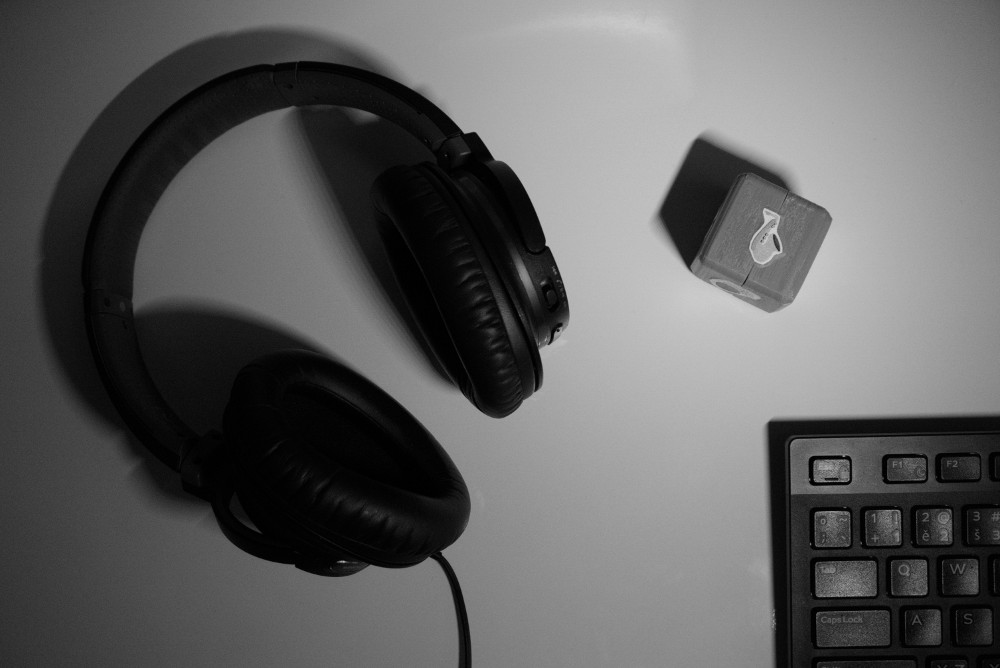
\includegraphics[scale=1.6]{cube2.jpg}
\caption{Minimalist design helps keep the user in focus.}
\label{fig:phones}
\end{figure}

\begin{figure}[H]
\centering
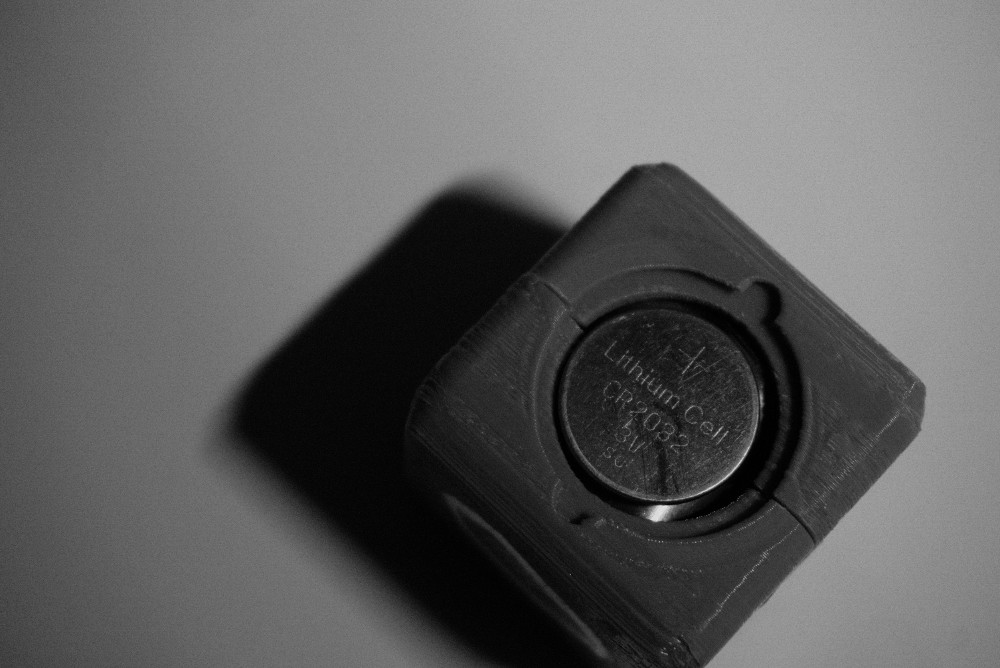
\includegraphics[scale=1.6]{battery_closeup.jpg}
\caption{The combination of 3D printing and parametric modelling allows for much-needed precision.}
\label{fig:battery}
\end{figure}

\newpage

\begin{thebibliography}{}
\bibitem{gravit}
GRAVIT GMBH. \textit{Gravit Designer} [online][visited on 2018-06-03]. Available from: \textit{https://designer.io/}
\bibitem{openscad}
KINTEL Marius. \textit{OpenSCAD - The Programmers Solid 3D CAD Modeller} [online][visited on 2018-06-03]. Available from: \textit{http://www.openscad.org/}
\bibitem{apple}
APPLE INC. \textit{iOS Human Interface Guidelines} [online][visited on 2018-06-03]. Available from: \textit{https://developer.apple.com/ios/human-interface-guidelines/overview/themes/}
\bibitem{emoji}
RANKS.COM, EMOJITWO COMMUNITY. \textit{Emojitwo} [online][visited on 2018-06-03]. Available from: \textit{https://emojitwo.github.io/}
\end{thebibliography}

\end{document}
